\lecture{18}{Phase Transformation of Mixtures}{Qiang Zhu}{scribe-name1,2,3}


\section{Free Energy of Mixture}
Phase Transformations become more complicated when a system contains two or more types of particles.
For example, what will happen if you lower the temperature of this mixture at 1 atm.
You might expect that all the oxygen will liquefy at 90.2 K, leaving a gas of pure nitrogen which 
would transform to liquid till 77.4 K. However, no liquid at all forms until the temperature drops to 81.6 K.
Similar behaviors happen on liquid-solid transition as well. How to understand it?

\begin{figure}[h]
\centering
\label{ideal-mix}
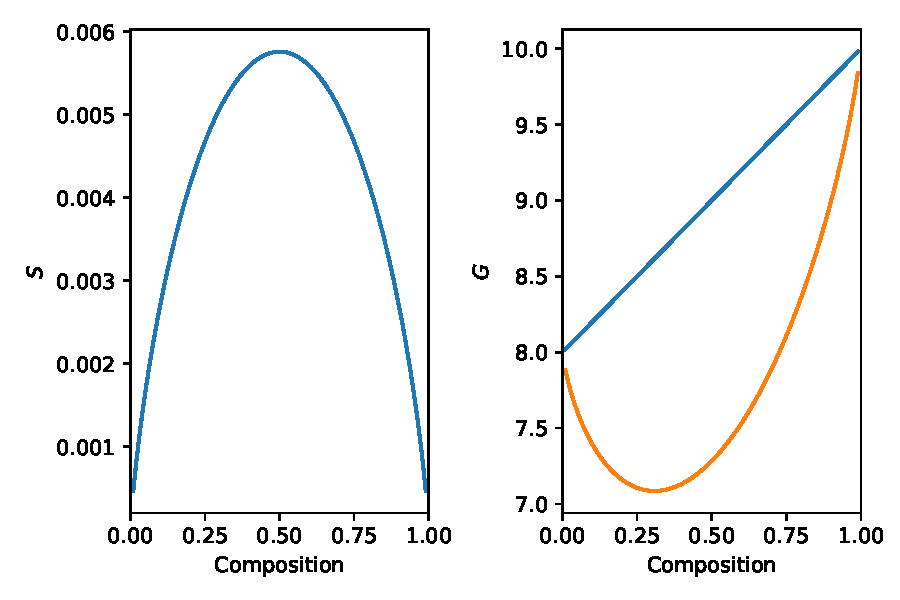
\includegraphics[width=12cm]{imgs/Ideal-Mixture.pdf}
\caption{The Phase diagram of ideal mixture, where $TS$ is the only term to contribute to $\Delta{G}$. }
\end{figure}


The key is to look at the Gibbs free energy as we did on vdW model. Let's consider a system of two molecules, $A$
and $B$, suppose that they are initially separated, sitting side by side at the same temperature and pressure. For
an unmixed system, the total free energy is just the sum of the two subsystems,
\begin{equation}
G = (1-x)G_A + xG_B,
\end{equation}
where $x$ is the fraction of $B$. 

Now suppose that we remove the partition between two sides and let them mix. From the definition of $G=U+PV-TS$.
\begin{enumerate}
\item $U$, depends on the intermolecular forces
\item $V$, depends on the forces as well
\item $S$, must increase according to what we learn in chapter 2.
\end{enumerate}

For the case of ideal gas (Fig. \ref{ideal-mix}), we can assume $U,V$ don't change.

Therefore the free energy of the mixture becomes,
\begin{equation}
G = (1-x)G_A + xG_B + RT[x\text{ln}x + (1-x)\text{ln}(1-x)]
\end{equation}

Note this only applies to ideal mixture. For real cases such as the mixing of liquids, it would usually cause the increase of $U$.

Let $n$ be the average number of the nearest neighbours, $\mu_0$ be the average potential energy of A-A or B-B interaction,
\begin{equation}
U = 1/2Nn\mu_0   
\end{equation}

If we mix it, the total potential energy then becomes,
\begin{equation}
\begin{split}
U &= 1/2[(1-x)N(xn\mu_\text{AB} + (1-x)n\mu_0) + xN(xn\mu_0 + (1-x)n\mu_\text{AB})] \\
  &= 1/2Nn([x^2+(1-x)^2]\mu_0 + 2x(1-x)\mu_\text{AB})
\end{split}
\end{equation}

Therefore,
\begin{equation}
\Delta{U} = Nnx(1-x)(\mu_{AB}-\mu_0)
\end{equation}

\begin{figure}[h]
\centering
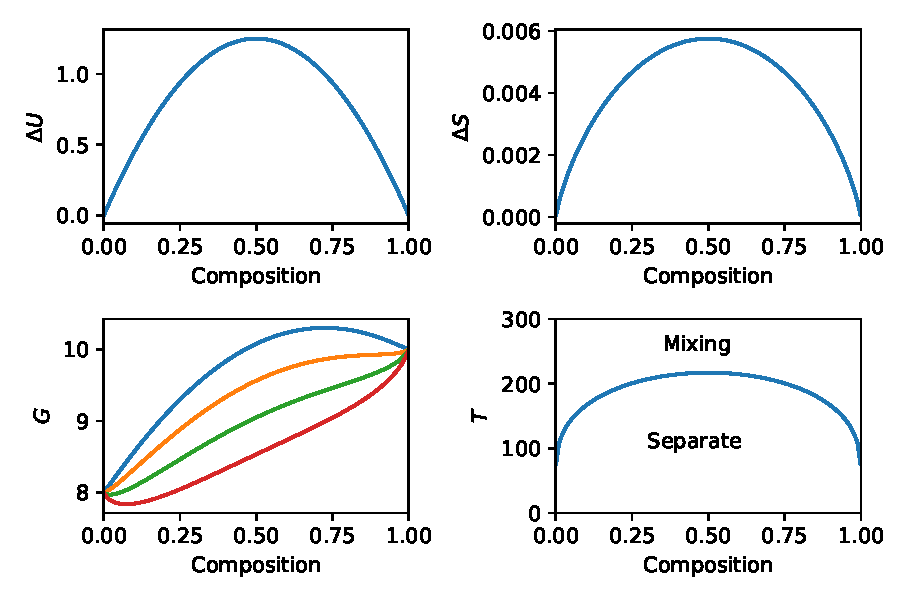
\includegraphics[width=12cm]{imgs/NonIdeal-Mixture.pdf}
\caption{The Phase diagram of non-ideal mixture, where only $\Delta{U}$ also contributes to $\Delta{G}$. When $\Delta{U}$ is positive, there exists 
a competition between $U$ and $TS$.}
\label{fig-non-ideal}
\end{figure}

The qualitative results are shown in Fig. \ref{fig-non-ideal}. If $\mu_{AB}$ is greater than $\mu_0$, it means $\Delta{U}$ favors the mixing. But it is not always the case. If $\mu_{AB}$ is smaller than $\mu_0$, there would be a competition between $U$ and $TS$. At low $T$, the shape is concave-down. At sufficiently high $T$, $TS$ becomes dominant, thus the shape is concave-up. But a concave-down free energy function indicates an unstable mixture. Therefore, we know $T$ determines if $\Delta{G}$ is positive or negative. For each given $x$ we can determine the critical temperature. Such a $T-x$ diagram could be very useful to help us identify which region the systems are miscible or not.

\begin{figure}[ht]
\centering
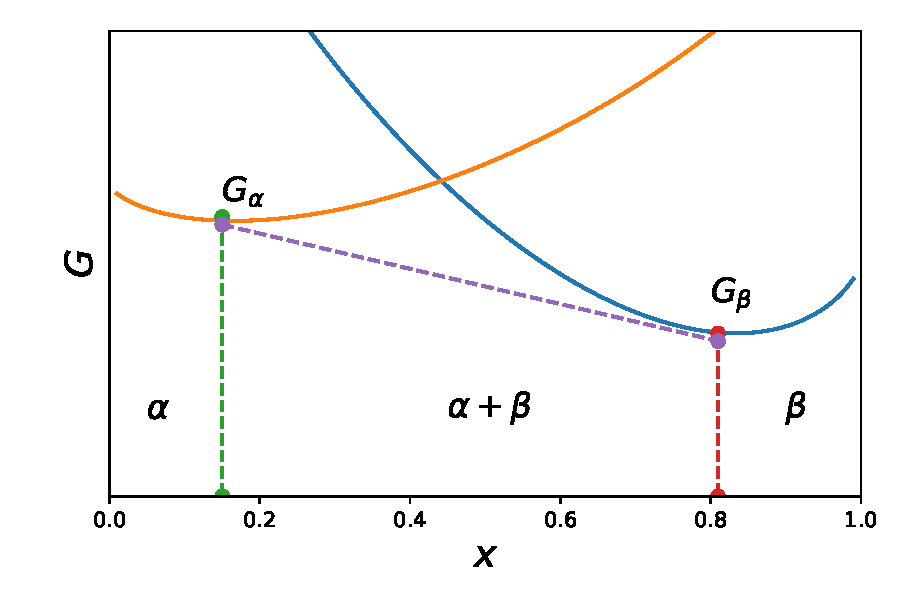
\includegraphics[width=10cm]{imgs/two-solids.pdf}
\label{fig-calc}
\caption{The Phase diagram of two systems which are not miscible to each other. In the intermediate region, the phase is a mixture of $\alpha$ and $\beta$.
This is called \textbf{solubility gap}.}
\end{figure}


\section{Phase diagram of a Miscible Mixture}
Let's come back to the problem of liquefy air. 
\begin{enumerate}
\item $T_A$, oxygen will start to liquefy at 90.2 K 
\item $T_B$, nitrogen will completely become liquid at 77.4 K. 
\item $T_A<T<T_B$, liquid and gas will coexist, depending on the ratio $x$.
\end{enumerate}

$G-x$ diagram\\
$T-x$ diagram\\
\begin{figure}[ht]
\centering
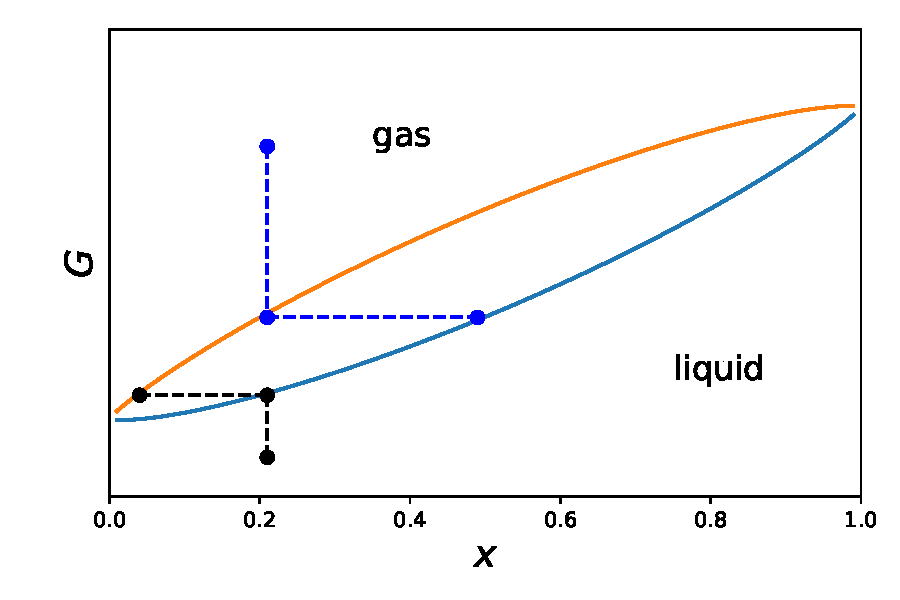
\includegraphics[width=10cm]{imgs/air.pdf}
\caption{The Phase diagram of air mixture.}
\end{figure}


\section{Phase Diagram of Eutectic Mixture}
Most two solids do not maintain the same crystal structures over the entire range of composition. If we consider the the solid-liquid transition with the possibility of two solid phases, this picture will become more complicated. Again the idea is to look at the free energy at various temperatures. Suppose $T_B$ is the melting point of B and $T_A$ is the melting point of A. 

\begin{enumerate}
    \item At high temperatures the free energy of the liquid will be below that of either solid phase. 
    \item As the temperature drops, all three energy functions will increase ($\frac{\partial G}{\partial T}=-S$), but the free energy of the liquid will increase fastest because it has higher $TS$ term. Below $T_B$ the liquid's free energy curve will intersect that of the B phase, so there is a range of compositions for which the stable configuration is an unmixed combination of liquid and B. 
    \item as T decreased further, this range reaches the A side of the diagram and you will find the range of an unmixed combination of liquid and A.
    \item if we drop the T further, we will find that A+liquid and B+liquid will meet at a particular point (\textbf{Eutectic point}). An Eutectic point defines the lowest melting point of the system. 
\end{enumerate}

\begin{figure}[ht]
\centering
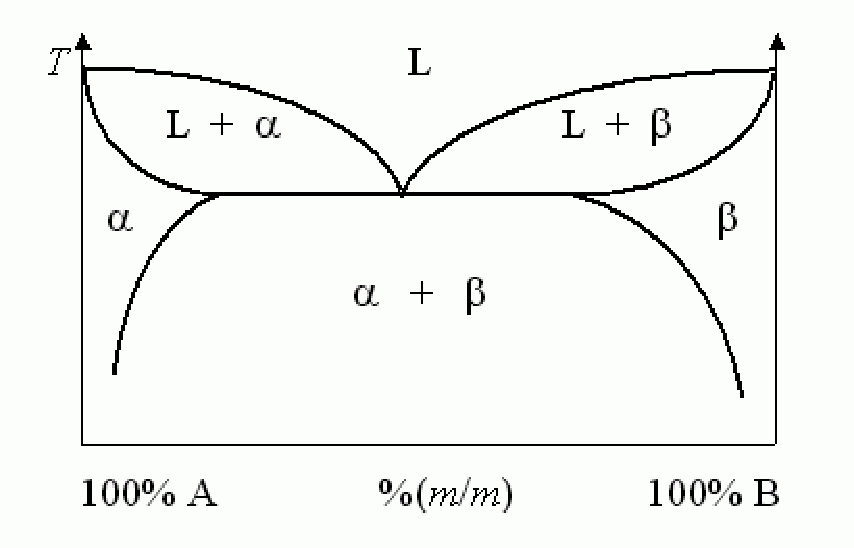
\includegraphics[width=10cm]{imgs/Eutectic.pdf}
\caption{The Phase diagram of A-B mixture.}
\end{figure}


